\documentclass[10,a4paperpaper,]{article}

  \title{Analysis and Forecast of Fish Trade Import and Export \break in
Norway using time features with Glmnet and Prophet}
  \author{Damien Dupré}
  \date{\today}
  


\newcommand{\logo}{dot_logo.png}
\newcommand{\cover}{dcu_cover.png}
\newcommand{\iblue}{2b4894}
\newcommand{\igray}{d4dbde}
\usepackage{ragged2e}

% Author: Karol KozioL
% License: GPL-3
% Modified by: Sarah Wagner

% % % packages -----------------------------------------------------------------------------------
\usepackage{amsmath}
\usepackage{array}
\usepackage{booktabs}
\usepackage{calc}
\usepackage{eso-pic}
\usepackage{fancyhdr}
\usepackage{fontspec}
\usepackage[left = 2.5cm, right = 2.5cm, top = 1.2cm, bottom = 1.2cm, includeheadfoot]{geometry}
\usepackage{graphicx}
\usepackage[utf8]{inputenc}
\usepackage{lastpage}
\usepackage{multirow}
\usepackage{tabularx} 
\usepackage{tikz}
\usepackage{titlesec}
\usepackage{xcolor, colortbl}

% % % settings -----------------------------------------------------------------------------------

% % custom colors
\definecolor{iblue}{HTML}{\iblue}
\definecolor{igray}{HTML}{\igray}

% definition of pagename
\newcommand\pagename{Page}

% % fonts 
\defaultfontfeatures{Mapping = tex-text}
\setmainfont[BoldFont = Lato-Bold.ttf, ItalicFont = Lato-Italic.ttf, BoldItalicFont = Lato-BoldItalic.ttf]{Lato-Regular.ttf}
\newfontfamily\headingfont[ItalicFont = Lato-BlackItalic.ttf]{Lato-Black.ttf}


% % sections
\titleformat{\section}{\color{iblue}\headingfont\Large\bfseries}{\thesection}{1em}{}[\titlerule]
\titleformat{\subsection}{\color{iblue}\headingfont\large\bfseries}{\thesubsection}{1em}{}
\titleformat{\subsubsection}{\color{iblue}\headingfont\bfseries}{\thesubsubsection}{1em}{}

% % misc
\setlength{\parindent}{0em} 
\linespread{1}
\raggedright
\newcolumntype{C}{>{\centering\arraybackslash}X}


% % % custom titlepage ----------------------------------------------------------------------------
\newcommand\BackgroundPic{%
	\put(0,0){%
		\parbox[b][\paperheight]{\paperwidth}{%
			\vfill
			\centering
			
\includegraphics[width=\paperwidth,height=\paperheight]{\cover}%
			\vfill
}}}

\makeatletter

% pagestyle titlepage
\fancypagestyle{customtitle}{
	\lhead{}
	\chead{}
	\rhead{}
	\makeatother
	\lfoot{}
	\cfoot{}
	\rfoot{
\includegraphics{\logo}}
}


% titlepage
\renewcommand{\maketitle}{
	\thispagestyle{customtitle}
	\AddToShipoutPicture*{\BackgroundPic}
	\ClearShipoutPicture
	
	\phantom{a}\hfill
	\vspace{14cm}
	
	\begin{tabular}[l]{@{}p{\textwidth}@{}}
		\color{iblue}\headingfont\LARGE\@title\\[1em]
		\color{iblue}\headingfont\large\@author\\[1em]
		\color{iblue}\headingfont\small\@date\\[1em]
	\end{tabular}
	
	
	
	\clearpage
}
\makeatother

% % % header and footer ---------------------------------------------------------------------------
\pagestyle{fancy}
\lhead{}
\chead{}
\rhead{ 
\includegraphics{\logo}}
\makeatother
\newlength{\myheight}
\lfoot{}
\cfoot{}
\rfoot{\pagename~\thepage \hspace{1pt} / \pageref{LastPage}}
\renewcommand\headrulewidth{0pt}
\renewcommand\footrulewidth{0pt}




\begin{document}


\renewcommand{\contentsname}{Analysis and Forecast of Fish Trade Import and Export in Norway}

\renewcommand{\pagename}{Page}


\maketitle
\tableofcontents
\addcontentsline{toc}{section}{Contents}
\clearpage
\justifying

\section{Introduction}

This report investigate the evolution of fish unit price and implement
algorithm to forecast this evolution. Each chapter is dedicated to a
specific fish trade analysis which involves a type of fish, a country
and its type of trade (import or export).

Within these chapters, a first section is dedicated to the analysis of
the trade history using classic methods and visualisations. A second
section is dedicated to the implementation of forecast algorithms.
Currently, 2 different forecast algorithm models are implemented: Glmnet
and Prophet.

\begin{itemize}
\item
  Glmnet is a generalized linear model via penalized maximum likelihood
  trained for forecast purpose. The regularization path is computed for
  the lasso or elasticnet penalty at a grid of values for the
  regularization parameter lambda. The algorithm is extremely fast, and
  can exploit sparsity in the input matrix \(x\).
\item
  Prophet is a procedure for forecasting time series data based on an
  additive model where non-linear trends are fit with yearly, weekly,
  and daily seasonality, plus holiday effects. It works best with time
  series that have strong seasonal effects and several seasons of
  historical data. Prophet is robust to missing data and shifts in the
  trend, and typically handles outliers well.
\end{itemize}

Finally additional analyses are presented in order to focus on specific
points of the analysis such as factors influencing the Unit Price
evolution, Seasonality and Trade evolution of specific partners.

\clearpage

\section{Horse Mackerel and Scomber Exports from Norway}

\subsection{Analysis}

Between 2012 and 2020, Norway has exported horse mackerel to 32
countries worldwide. Data for Scomber are substantially different.
Indeed, between 1998 and 2019, Norway has exported Scomber to 108
countries worldwide.

The data collected shows a important discrepancy between these countries
regarding the trade history, the level of the price applied and its
volatility.

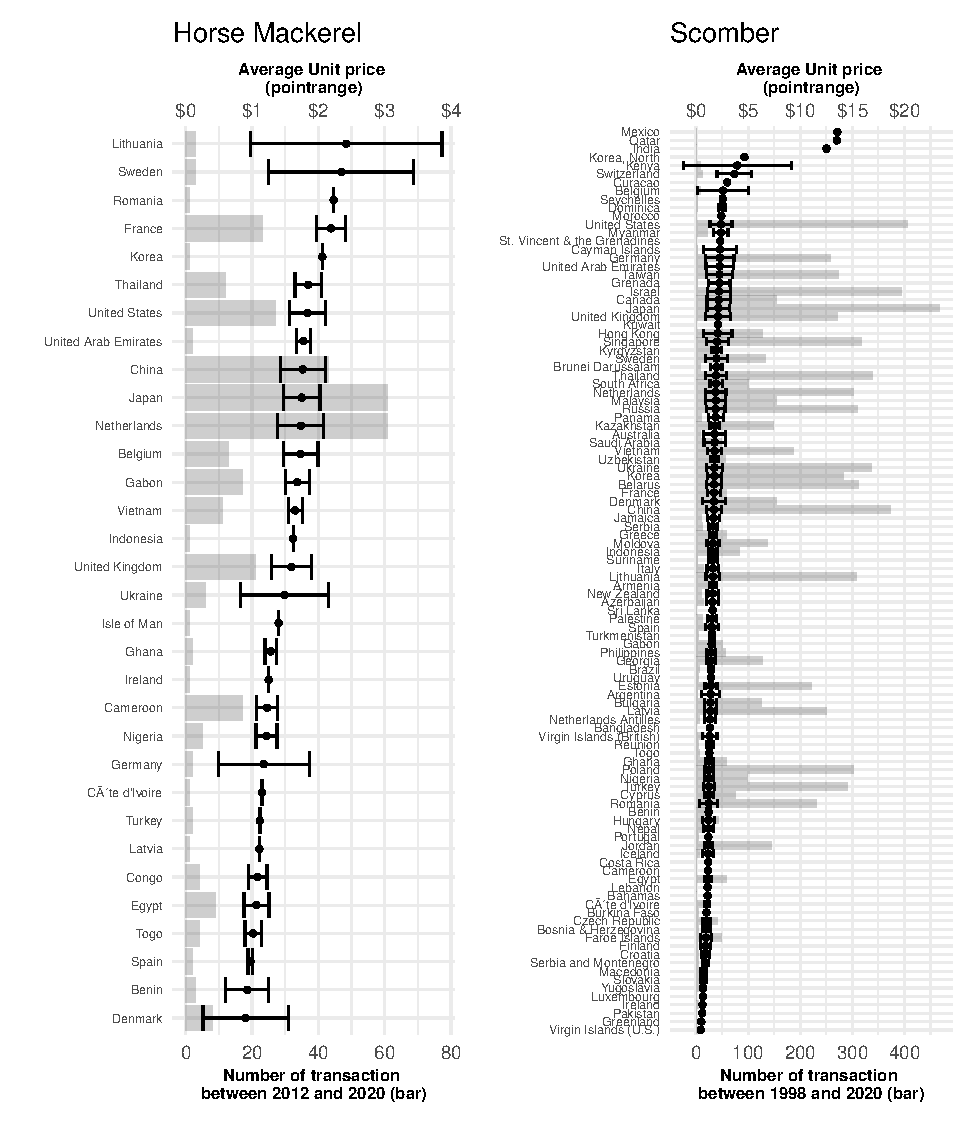
\includegraphics{report_files/figure-latex/unnamed-chunk-1-1.pdf}

In the Figure here above, it is possible to distinguish two different
patterns for Horse Mackerel and Scomber fish exports.

For Horse Mackerel trades, countries with a high average price and high
volatility such as Lithuania, high average price and low volatility such
as France, low average price and high volatility such as Denmark and low
average price with low volatility such as Egypt. A second factor is
particularly important to take into account, the level of trade can vary
between the countries. Some countries have only one or two trades while
others have more than 60 trades.

For Scomber, the lower Unit Price of the trade is the less volatility
there is expect for Mexico, Qatar and India but these countries have
only one trade and can be considered as outliers. It is interesting to
observe that the number of transaction according the countries does not
influence the average unit price.

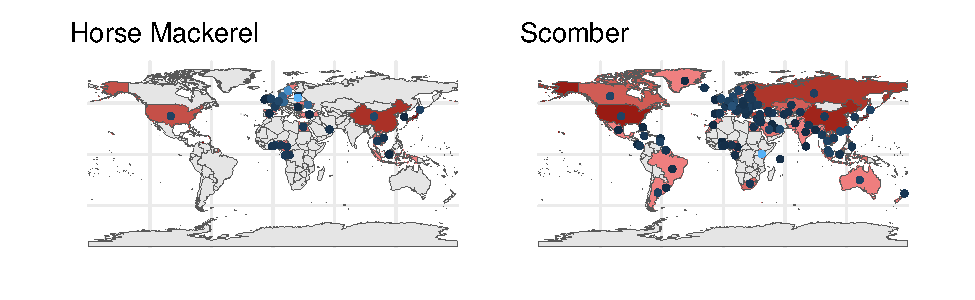
\includegraphics{report_files/figure-latex/unnamed-chunk-2-1.pdf}

The world map representations are summaries of the pointrange/bar plot
visualisation of the export trades. The red colour indicates the number
of trades (dark red means important trade history) while the blue dot
indicates the volatility in the trade (light blue means high
volatility). This representation show that there are significant
discrepancies between the export countries regardless their distance
from Norway or their continent.

Despite these significant differences between trade partners, for the
forecast models done in the next sections this bias will not be removed
as all the data will be taken into account. The available data are too
low in term of sampling frequency (once a month maximum), on a too short
period, with not enough data per country. Therefore an analysis country
wise is impossible. All the data will be taken into account in the
coming sections.

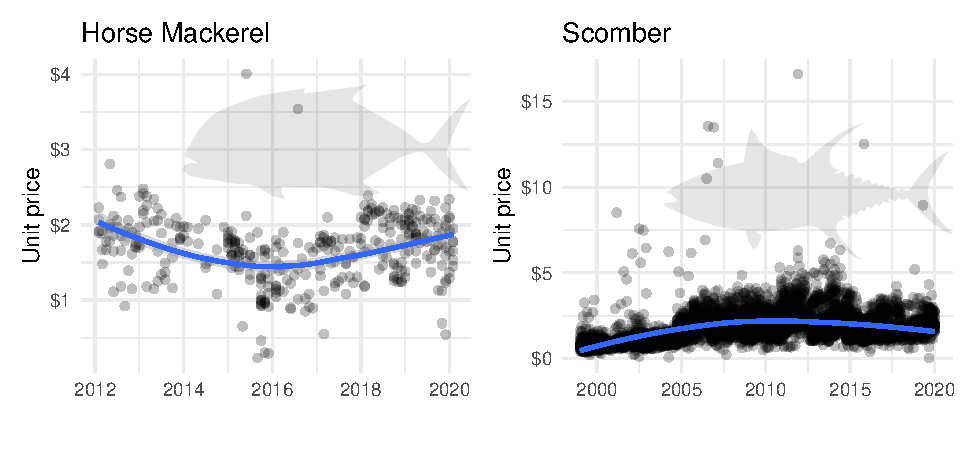
\includegraphics{report_files/figure-latex/unnamed-chunk-3-1.pdf}

The trend of the evolution of Horse Mackerel unit price since 2012
indicates following a slight parabolic inverse trend with a valley
(negative peak) in 2016 whereas the trend of the evolution of Scomber
unit price since 1998 indicates following a slight parabolic normal
trend with a peak around 2010.

\subsection{Glmnet Algorithm Forecast}

In order to forecast the evolution of fish price according the time, the
existing data are split in two sections: the train region which will be
used to build the forecast model and the test region which will be used
compare the data predicted with the actual data.

In order to process this forecasting model, 224 time features are
extracted and used to predict the evolution of the Horse Mackerel unit
price and 224 time features are extracted and used to predict the
evolution of the Scomber unit price.

By selecting a test region corresponding to the last two years (i.e.,
from 2018 to 2020), it is possible to compare the forecast accuracy with
the actual Average unit price values. The most used indicators are
\(RMSE\) and \(MAE\). Root Mean Square Error (RMSE) is the standard
deviation of the residuals (prediction errors). Residuals are a measure
of how far from the regression line data points are; RMSE is a measure
of how spread out these residuals are. In other words, it tells you how
concentrated the data is around the line of best fit. Mean Absolute
Error (MAE) is a measure of errors between paired observations
expressing the same phenomenon. This is known as a scale-dependent
accuracy measure and therefore cannot be used to make comparisons
between series using different scales. The closer to 0 is the \(RMSE\)
and \(MAE\) value, the better. In parallel, the \(R^2\) indicator also
ranges from 0 to 1 but the closer to 1 is the value, the better.

Here, for Horse Mackerel unit price prediction: \(RMSE_{hm} =\) 0.47 and
\(MAE_{hm} =\) 0.43. These results are encouraging but could be largely
be improved. The model explains \(R^2_{hm} =\) 3\% of the variance of
the Horse Mackerel unit price variation.

For the Scomber unit price prediction: \(RMSE_{sc} =\) 0.64 and
\(MAE_{sc} =\) 0.6. These results are not as good as those for the Horse
Mackerel and is explain by the amount of data available and their larger
variability. The model explains \(R^2_{sc} =\) 2\% of the variance of
the Scomber unit price variation.

Based on the model previously test, a forecast of the 24 next months is
performed. Even if the accuracy of the forecast model on the test table
is low, it is still possible to use it to forecast the price within 2
years.

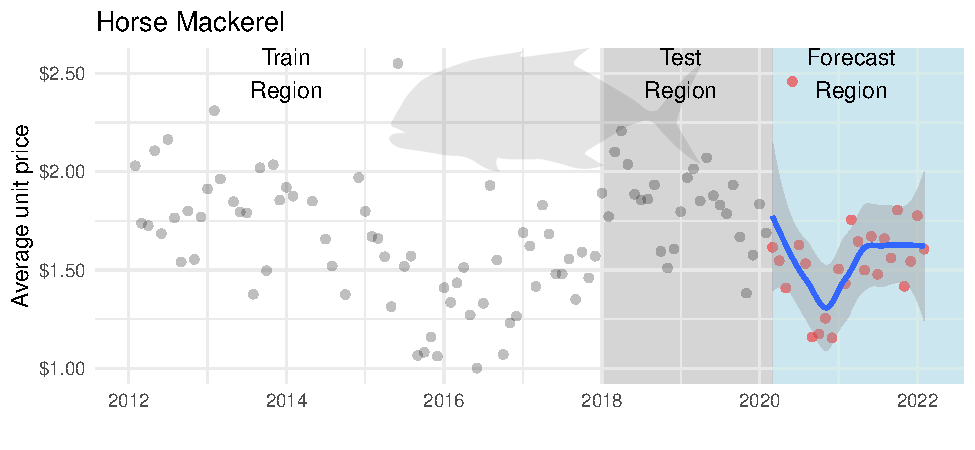
\includegraphics{report_files/figure-latex/unnamed-chunk-5-1.pdf}

In the case of the Horse Mackerel unit price prediction, The model
reveals a sharp decrease in 2020 and a rebound from 2021 followed by a
stabilization of the prices at \$1.60.

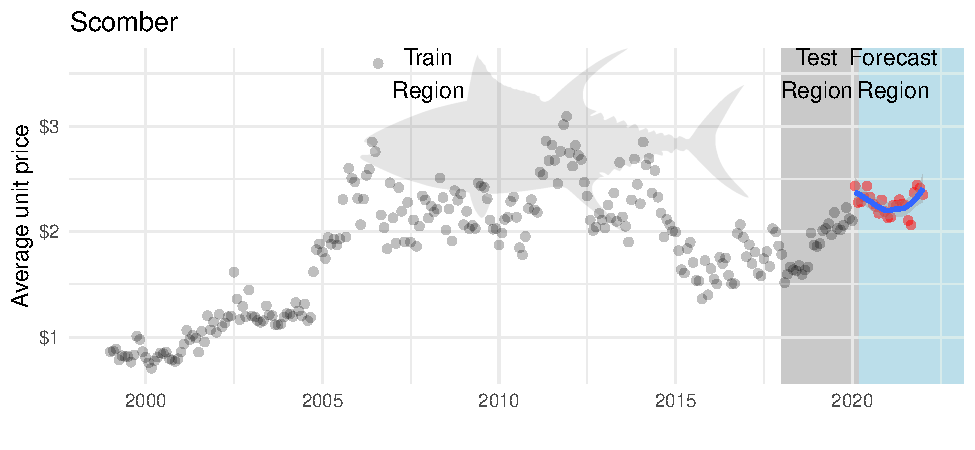
\includegraphics{report_files/figure-latex/unnamed-chunk-6-1.pdf}

In the case of the Scomber unit price prediction, The model reveals a
moderate decrease in 2020 and a rebound from 2021.

\subsection{Prophet Algorithm Forecast}

As the glmnet algorithm, the prophet decomposition extract the temporal
trends, seasonality, multiplicative factor and their prediction
residuals.

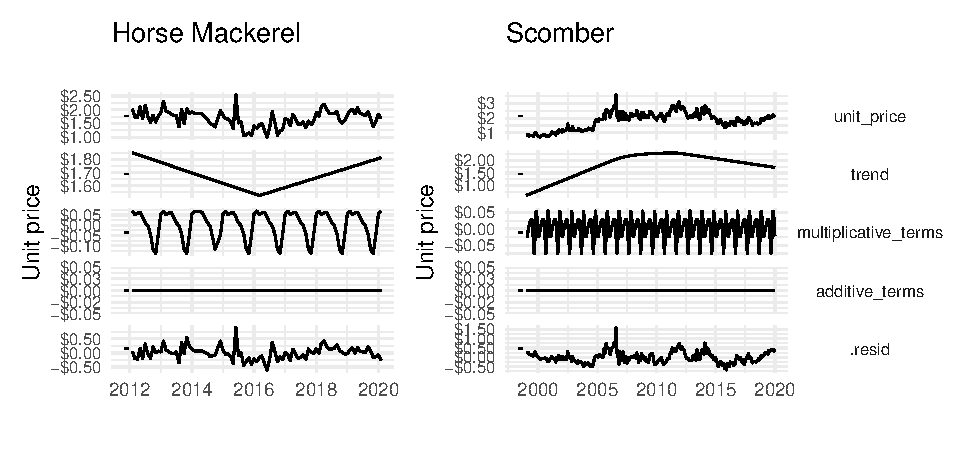
\includegraphics{report_files/figure-latex/unnamed-chunk-7-1.pdf}

In term of algorithm validation \(RMSE\) and \(MAE\) can be calculated
from the original data. For Horse Mackerel prediction, \(RMSE_{hm} =\)
0.57 and \(MAE_{hm} =\) 0.54, which is better than the glmnet algorithm.
For Scomber prediction, \(RMSE_{sc} =\) 0.39 and \(MAE_{sc} =\) 0.32.

The result of the forecast by Prophet uses the seasonality of the price
evolution (see Additional Analyses section) as well as the overall
trend.

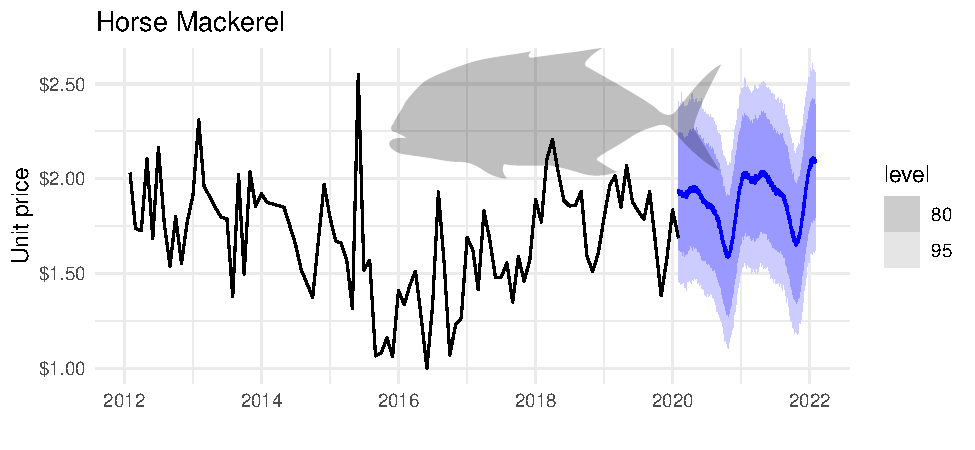
\includegraphics{report_files/figure-latex/unnamed-chunk-9-1.pdf}

For Horse Mackerel, the prediction reveals a decrease of the fish price
from February to November with a price in 2022 slightly higher than
2021.

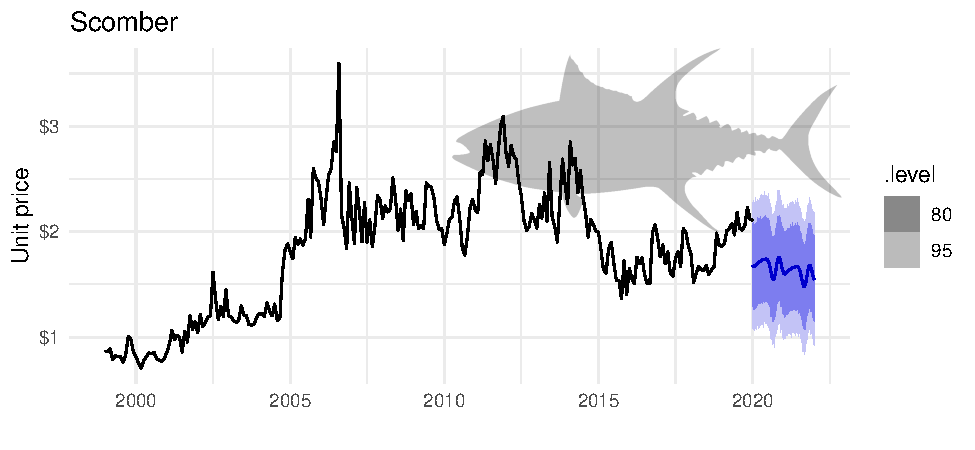
\includegraphics{report_files/figure-latex/unnamed-chunk-10-1.pdf}

For Scomber, the prediction reveals a decrease of the fish price until
2022 with seasonal changes.

\subsection{Additional Analyses}

The difference between countries that are historic and recurrent trade
partner with countries who have only several past trade is highly
relevant. Indeed we can imagine that price establishment is build on a
commercial relationship between the countries, if a country has no
history, the average price paid is likely to be higher than historical
trade partners which will bias the forecast of the evolution.

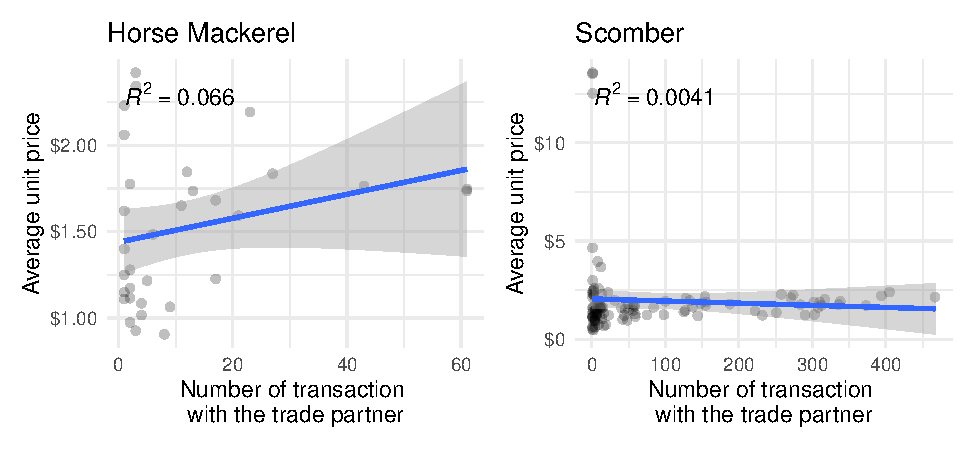
\includegraphics{report_files/figure-latex/unnamed-chunk-11-1.pdf}

However the results show that the number of trade has no significant
relationship with the average unit price of Horse Mackerel trade
(\(R^2 = .07\), \(F(1, 30) = 2.12\), \(p = .156\)) and Scomber trade
(\(R^2 = < .01\), \(F(1, 106) = 0.44\), \(p = .509\)).

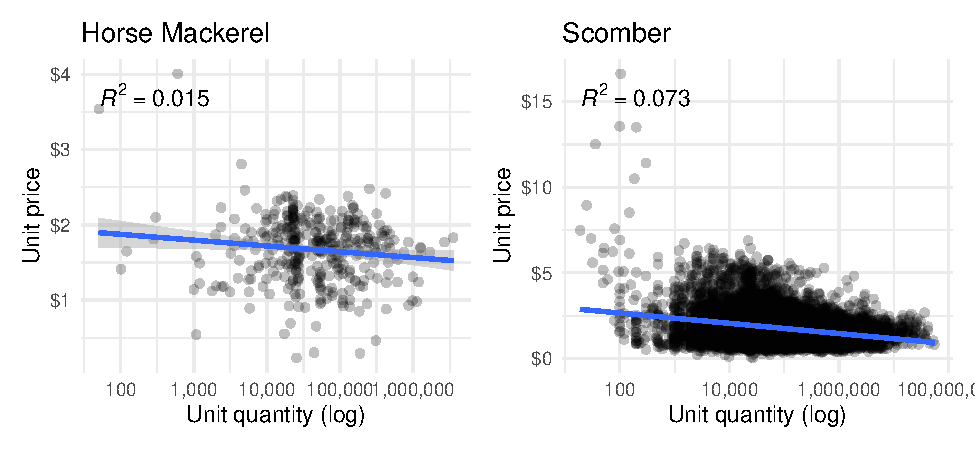
\includegraphics{report_files/figure-latex/unnamed-chunk-12-1.pdf}

Another possible bias involved in trade relationship is the possible
relationship between quantity and unit price. It seems logical to
believe that countries buying more will have more leverage to negotiate
their unit price. The results reveals a weak but significant
relationship between the unit quantity ordered on a log scale and Horse
Mackerel unit price (\(R^2 = .02\), \(F(1, 366) = 5.68\), \(p = .018\))
as well as Scomber unit price (\(R^2 = .07\), \(F(1, 9268) = 734.25\),
\(p < .001\)).

A future investigation would be to try to understand the factors
explaining why certain countries have a high average price and others a
low average price (beside the the number of trade).

\clearpage

\section{Horse Mackerel and Scomber Imports by Norway}

\subsection{Analysis}

Between 2012 and 2019, Norway has imported Horse Mackerel from 9
countries worldwide. Data for Scomber are substantially different.
Indeed, between 1999 and 2020, Norway has imported Scomber from 26
countries worldwide.

Similarly as the export, the data collected shows a important
discrepancy between these countries regarding the trade history, the
level of the price applied and its volatility.

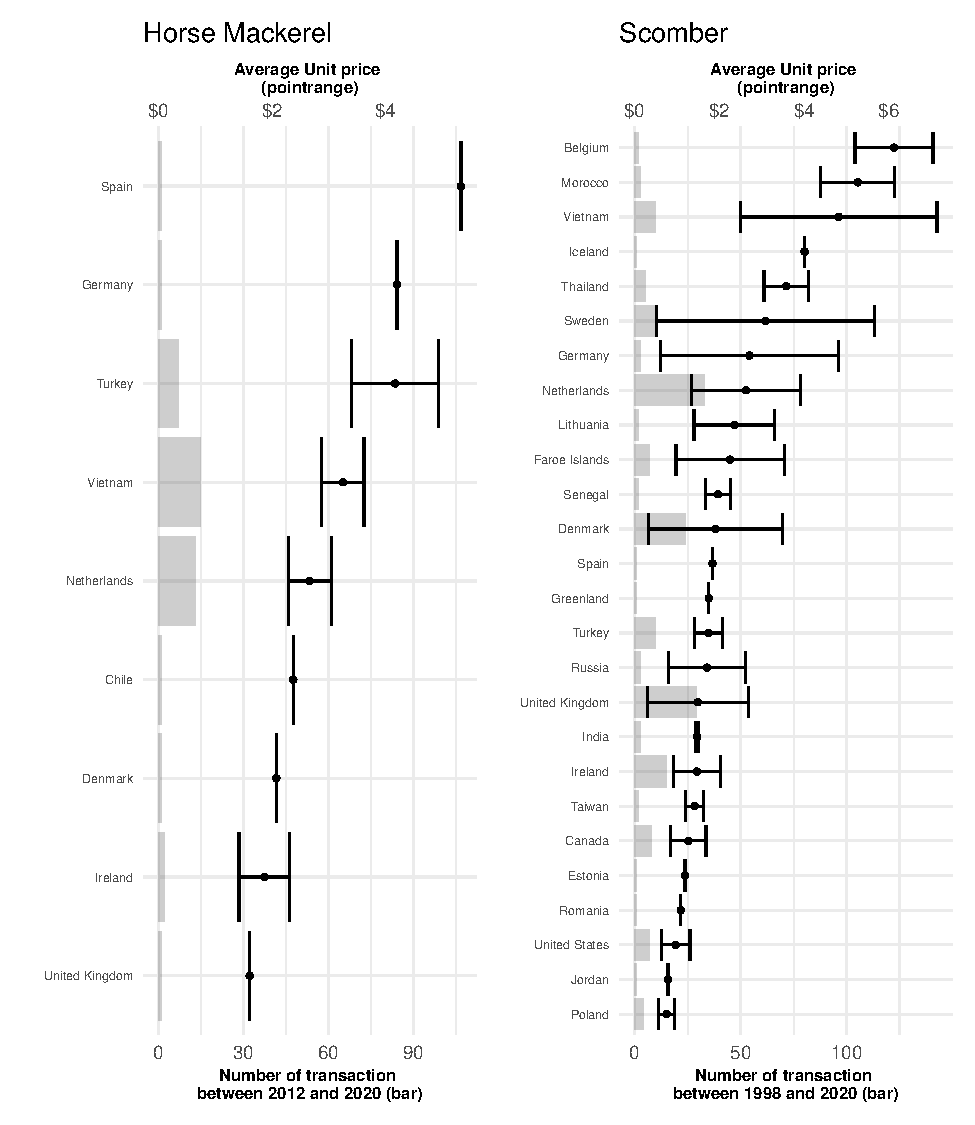
\includegraphics{report_files/figure-latex/unnamed-chunk-13-1.pdf}

For Horse Mackerel trades, countries with a high average price and high
volatility such as Turkey, Vietnam and the Netherlands, high average
price and low volatility such as Spain and Germany, low average price
and high volatility such as Ireland and low average price with low
volatility such as the United Kingdom. In a similar way as the export of
Horse Mackerel, the level of trade can vary between the countries and is
particularly important to take into account. Some countries have only
one or two trades while others have more than 20 trades.

For Scomber, it is possible to identify the same pattern: - high price/
high volatility (such as Vietnam) - high price/ low volatility (such as
Belgium and Morocco) - low price/ high volatility (such as the United
States) - low price/ low volatility (such as Jordan and Romania)

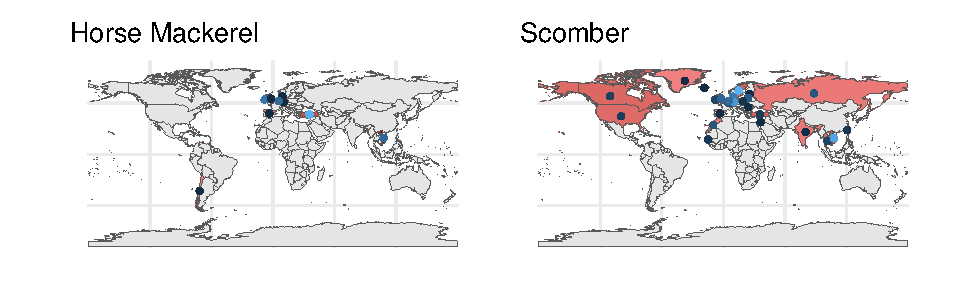
\includegraphics{report_files/figure-latex/unnamed-chunk-14-1.pdf}

The world map representations are summaries of the pointrange/bar plot
visualisation of the import trades. The red colour indicates the number
of trades (dark red means important trade history) while the blue dot
indicates the volatility in the trade (light blue means high
volatility). This representation show that there are significant
discrepancies between the type of fish in term of country partner and
trading history.

In a similar way as it has been done for the export forecast, all the
data will be taken into account in the coming sections. Specific effects
and characteristic of countries will not be taken into account and an
average unit price per month is applied for the overall trade partners.

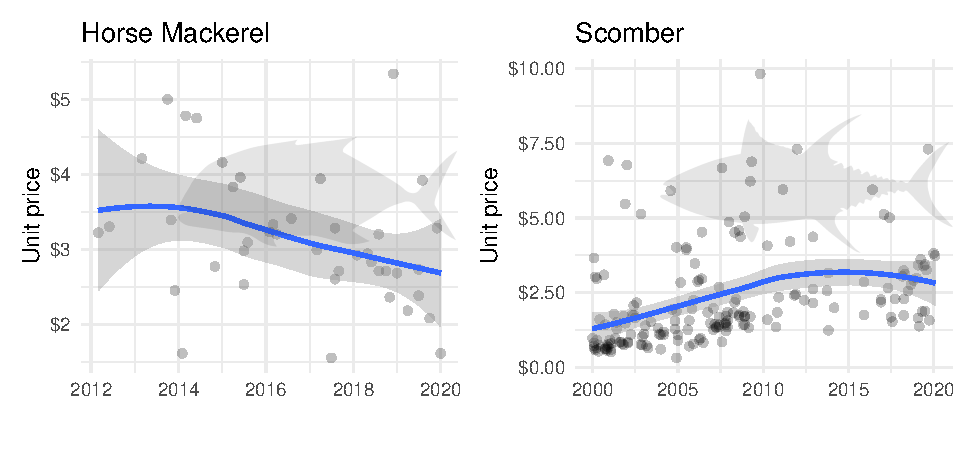
\includegraphics{report_files/figure-latex/unnamed-chunk-15-1.pdf}

The trend of the evolution of Horse Mackerel unit price since 2012
indicates a slow but continuous decrease whereas the trend of the
evolution of Scomber unit price since 1999 increased since 2000 and are
now stabilized with a slight decrease.

\subsection{Glmnet Algorithm Forecast}

In order to forecast the evolution of fish price according the time, the
existing data are split in two sections: the train region which will be
used to build the forecast model and the test region which will be used
compare the data predicted with the actual data.

In order to process this forecasting model, 224 time features are
extracted and used to predict the evolution of the Horse Mackerel unit
price and 224 time features are extracted and used to predict the
evolution of the Scomber unit price.

By selecting a test region corresponding to the last two years (i.e.,
from 2018 to 2020), it is possible to compare the forecast accuracy with
the actual Average unit price values. The most used indicators are
\(RMSE\) and \(MAE\). Root Mean Square Error (RMSE) is the standard
deviation of the residuals (prediction errors). Residuals are a measure
of how far from the regression line data points are; RMSE is a measure
of how spread out these residuals are. In other words, it tells you how
concentrated the data is around the line of best fit. Mean Absolute
Error (MAE) is a measure of errors between paired observations
expressing the same phenomenon. This is known as a scale-dependent
accuracy measure and therefore cannot be used to make comparisons
between series using different scales. The closer to 0 is the \(RMSE\)
and \(MAE\) value, the better. In parallel, the \(R^2\) indicator also
ranges from 0 to 1 but the closer to 1 is the value, the better.

Here, for Horse Mackerel unit price prediction: \(RMSE_{hm} =\) 1.03 and
\(MAE_{hm} =\) 0.8. These results reveals that this prediction could be
largely be improved. The differences between the months make this
prediction model very difficult to establish. The model explains
\(R^2_{hm} =\) 3\% of the variance of the Horse Mackerel unit price
variation.

For the Scomber unit price prediction: \(RMSE_{sc} =\) 1.52 and
\(MAE_{sc} =\) 1.04. These results are once again not as good as those
for the Horse Mackerel. The trading of Scomber appear to be particularly
difficult. The model explains \(R^2_{sc} =\) 2\% of the variance of the
Scomber unit price variation.

Based on the model previously test, a forecast of the 24 next months is
performed. Even if the accuracy of the forecast model on the test table
is low, it is still possible to use it to forecast the price within 2
years.

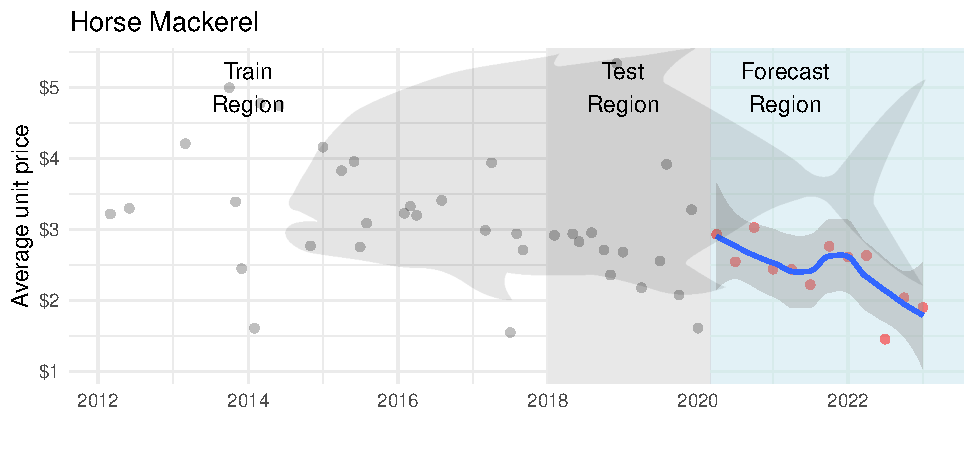
\includegraphics{report_files/figure-latex/unnamed-chunk-17-1.pdf}

In the case of the Horse Mackerel unit price prediction, The model
reveals a slow decrease until 2024 followed by a rebound.

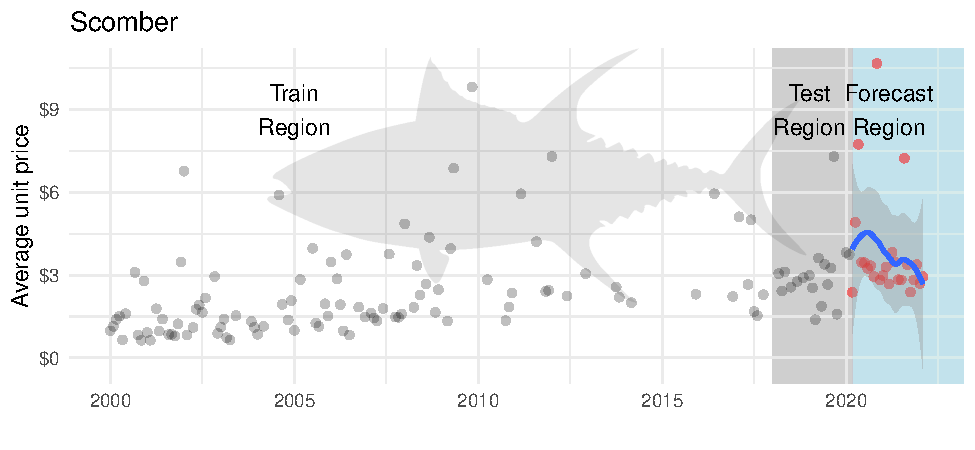
\includegraphics{report_files/figure-latex/unnamed-chunk-18-1.pdf}

In the case of the Scomber unit price prediction, The model reveals a as
significant increase in first 6 months of 2020 and a continuous decrease
until 2022.

\subsection{Prophet Algorithm Forecast}

As the glmnet algorithm, the prophet decomposition extract the temporal
trends, seasonality, multiplicative factor and their prediction
residuals.

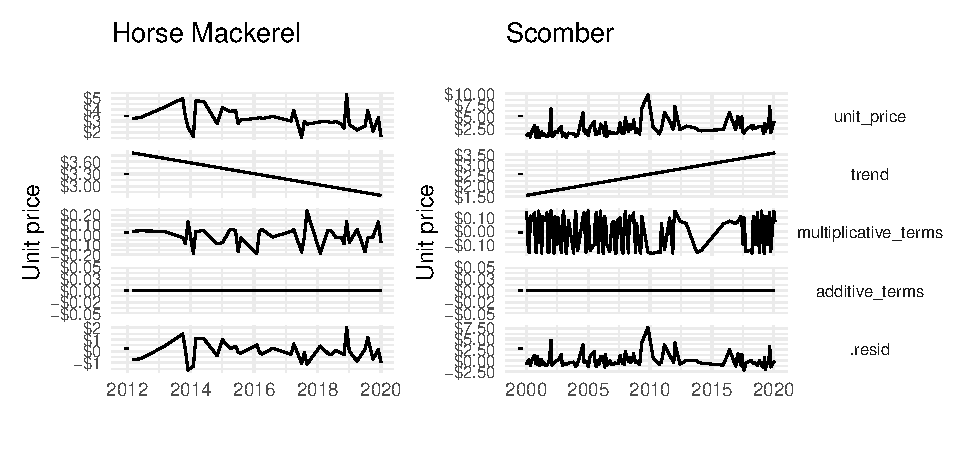
\includegraphics{report_files/figure-latex/unnamed-chunk-19-1.pdf}

In term of algorithm validation \(RMSE\) and \(MAE\) can be calculated
from the original data. For Horse Mackerel prediction, \(RMSE_{hm} =\)
1.18 and \(MAE_{hm} =\) 0.78, which is not as good as the glmnet
algorithm. For Scomber prediction, \(RMSE_{sc} =\) 1.73 and
\(MAE_{sc} =\) 1.53 which is again higher than those from the glmnet
algorithm.

The result of the forecast by Prophet uses the seasonality of the price
evolution (see Additional Analyses section) as well as the overall
trend.

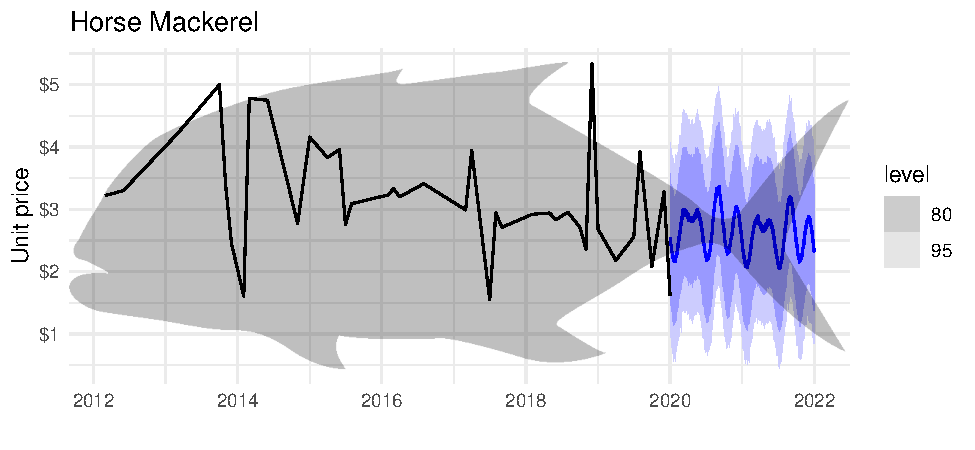
\includegraphics{report_files/figure-latex/unnamed-chunk-21-1.pdf}

For Horse Mackerel, the prediction reveals a high seasonal effect with a
stationary trend.

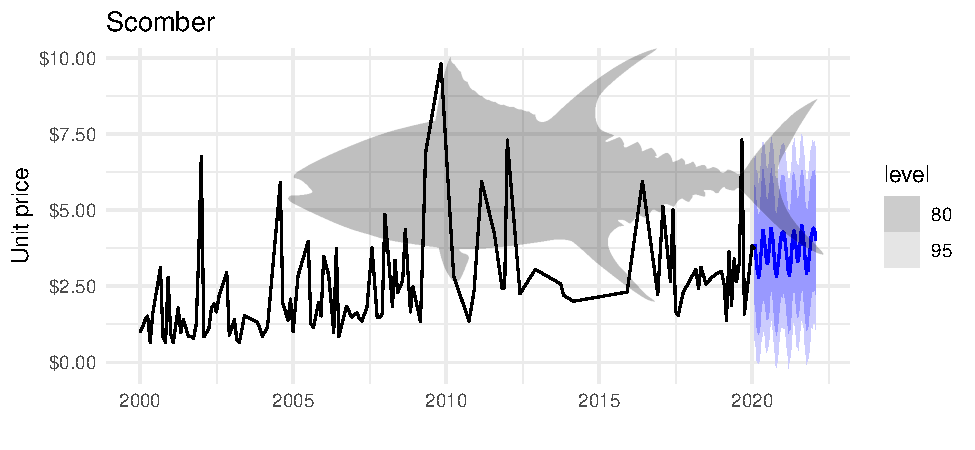
\includegraphics{report_files/figure-latex/unnamed-chunk-22-1.pdf}

For Scomber, the prediction reveals a high seasonality effect as well
but the trend shows a significant increase according the time.

\subsection{Additional Analyses}

A linear regression was performed between the average unit price and the
number of transaction with a trade partner for Horse Mackerel and
Scomber in order to highlight possible factors to be taken into account.

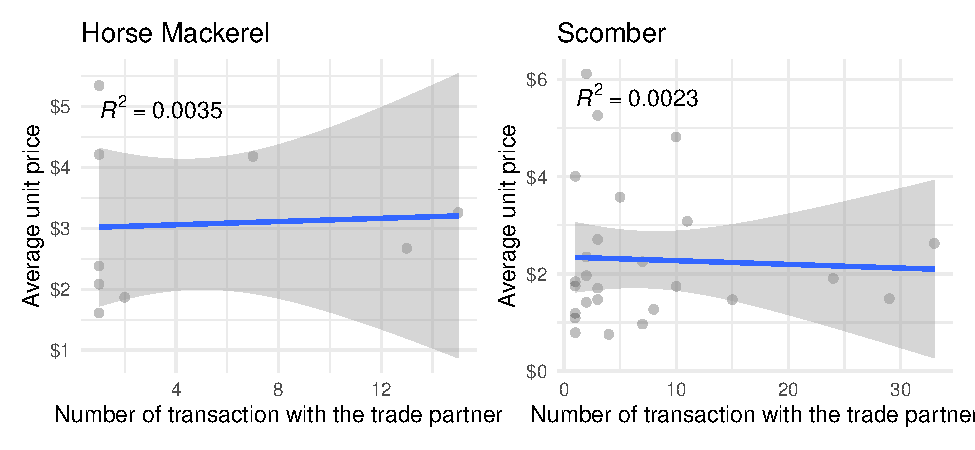
\includegraphics{report_files/figure-latex/unnamed-chunk-23-1.pdf}

However the results show that the number of trade has no significant
relationship with the average unit price of Horse Mackerel trade
(\(R^2 = < .01\), \(F(1, 7) = 0.02\), \(p = .880\)) and Scomber trade
(\(R^2 = < .01\), \(F(1, 24) = 0.05\), \(p = .818\)).

Another possible bias involved in trade relationship is the possible
relationship between quantity and unit price.

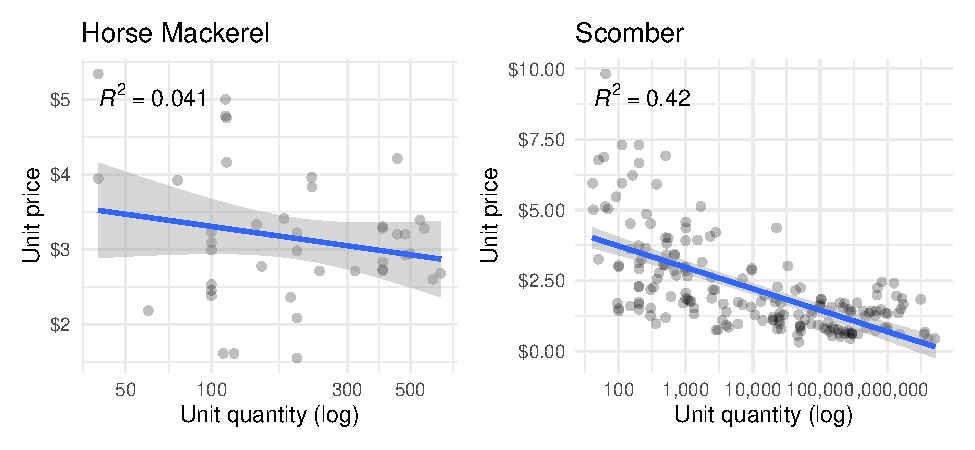
\includegraphics{report_files/figure-latex/unnamed-chunk-24-1.pdf}

Interestingly, the results reveals a non significant relationship
between the unit price and the the quantity traded for Horse Mackerel
(\(R^2 = .04\), \(F(1, 40) = 1.73\), \(p = .196\)) but as strong and
significant relationship between the unit price and the the quantity
traded for Scomber (\(R^2 = .42\), \(F(1, 187) = 133.41\),
\(p < .001\)). This last results reveals the important differences in
the trade of this two different fishes.

\clearpage

\section{Conclusion}

In the previous sections of this document have been presented the
analysis and forecast of Horse Mackerel and Scomber unit price in export
and import trades by Norway. The analysis of this evolutions reveals
similarities between the fishes and between the types of trade
(i.e.~export vs.~import). The analysis also revealed the differences
between the trade partners in term of trade history and their negotiated
unit price (specific averages and volatility indexes). For the purpose
of this forecast analysis an average unit price per month was calculated
in order to remove the influence of trade history between the different
partners.

In order to forecast the evolution of Horse Mackerel and Scomber unit
price in export and import trades by Norway, two specific algorithm were
applied: Glmnet and Prophet. These algorithms were using time features
and properties of the time series to perform this forecasting according
the time. Through some visualisations, the forecast of the unit price
over 24 months was revealed.

In addition to the forecast, validity indicators were calculated. As
this report is a presentation of preliminary results of this forecasting
work, these indicators revealed the necessity to improve the validity of
this forecast. However, this results is not surprising as the building
of forecasting models to predict high volatility financial time-series
requires years to build as well as infrastructures and findings.

Beside the necessity for more time in the exploration of suitable
algorithms and factors to take into account, this analysis could be
improved by increasing the quality of the data used (time span, time
resolution, trading partner network, type of fishes) and by increasing
the processing power in the analysis (increase of features and variable
to take into account).

Despite these limitations, this report has highlight the possibility to
built forecasting models a minima and built established a framework for
future improvements.


\end{document}
